\chapter{COMET Phase-I Sensitivity and Background Estimates}

With the framework to simulate backgrounds from atmospheric muons in place, we
can now combine the results into a complete sensitivity and background
simulation study for COMET Phase-I. In this chapter, we discuss our simulation
samples consisting of signal, decay in orbit (DIO), and atmospheric events, and
present our resulting expectations of the performance of Phase-I.

\section{Data samples}
Three simulation samples are produced for this study. A $\mu$--$e$ conversion
sample, a DIO sample and an atmospheric muon sample. All three are simulated in
the geometrical world shown in Figure~\ref{fig:bmc_geometry}. This geometry
differs from the older TDR design~\cite{the_comet_collaboration_comet_2020} by
the number of counters in the CTH. Here, each layer of the CTH has 64 counters
instead of the original 48, which mainly affects the detector's geometrical
acceptance. In addition, the outer layer of the CTH is composed of plastic
scintillation counters rather than the originally planned Cherenkov counters. As
we shall see, this has an important effect on the detector's ability to
discriminate atmospheric anti-muons from conversion electrons.

\subsection{\texorpdfstring{$\mu$--$e$}{Muon to electron} conversion} 

\subsubsection{Sample}

The signal sample is the most straightforward to produce. We initially generate
primary electrons with energy $E=\SI{104.97}{\MeV}$ uniformly inside the
stopping target disks. Their direction is isotropically distributed, as would be
the case in the conversion process. A uniform position distribution in each disk
is not realistic, because the actual distribution depends on where in the
stopping target the muons in the beam come at rest. To account for this, the
events are weighted according to the stopping positions of muons recorded in the
MC5 simulation. The weighting factor is determined from the relative probability
for a muon to stop at the sampled position, which is estimated by histogramming
the stopping positions in each disk.
Figure~\ref{fig:stopping_position_reweighting} shows the initially-sampled
uniform position distribution, the muon stopping position distribution from MC5,
and the result of event weighting. In total, $N_\mathrm{signal} =
2\times 10^6$ events are simulated to compose the signal sample.

% After applying geom cut of CTH trigger, how many remain?

\begin{figure}
    \centering
    \begin{subfigure}[t]{0.329\textwidth}
        \centering
        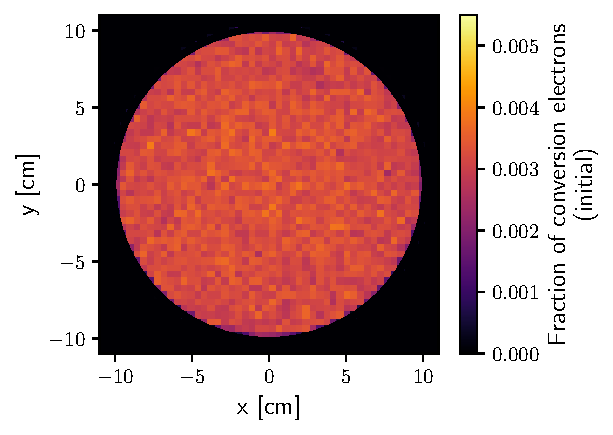
\includegraphics[width=\textwidth]{chapter6/initial_conversion_position_distribution.pdf}
        \caption{Pre-weighting.}
    \end{subfigure}
    \hfill
    \begin{subfigure}[t]{0.329\textwidth}
        \centering
        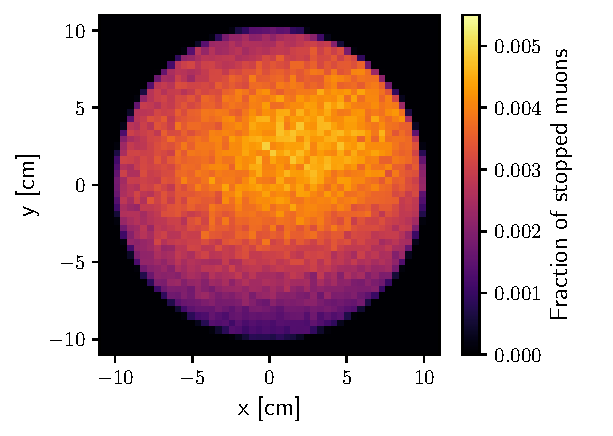
\includegraphics[width=\textwidth]{chapter6/stopped_muon_distribution.pdf}
        \caption{Bound muon position distribution from MC5 used as weight.}
    \end{subfigure}
    \hfill
    \begin{subfigure}[t]{0.329\textwidth}
        \centering
        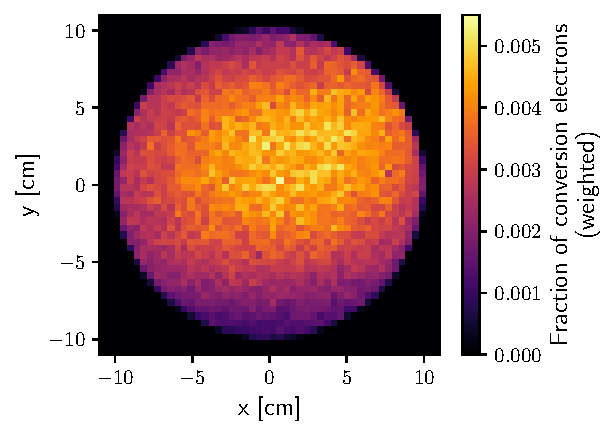
\includegraphics[width=\textwidth]{chapter6/weighted_conversion_position_distribution.pdf}
        \caption{Post-weighting.}
    \end{subfigure}
    \caption{ Initial position distribution of signal electrons before and after
        weighting them by the likelihood of a muon being bound in each bin. }
    \label{fig:stopping_position_reweighting}
\end{figure}


\subsubsection{Selection}
Signal events are selected based on detector acceptance criteria. We first
require fourfold coincidence in the CTH. Figure~\ref{fig:cydet_signal_event}
shows an example of a conversion event which passes this trigger criterion. The
fraction of events remaining defines the geometrical acceptance 
$$
A_\mathrm{geom} \equiv  \frac{\text{fourfold coincidences}}{N_\mathrm{signal}}.
$$
In this simulation, the estimated geometrical acceptance is $A_\mathrm{geom} =
\SI{21}{\percent}$. In comparison, the TDR cites $A_\mathrm{geom} =
\SI{26}{\percent}$ with the previous design of the CTH.


% Reconstruction
We do not fully simulate the reconstruction of signal electron trajectories in
the CDC. In order to approximate the effect of reconstruction uncertainties, a
smearing is applied to the true momentum of each track. The reconstructed
momentum is estimated as $p_r = p_t + x$, where $p_t$ is the true momentum of
the electron as it enters the CDC, $x \sim \mathcal{N}(0, \sigma)$, and $\sigma
= \SI{200}{\keV/\clight}$ is the expected momentum resolution of the CDC. Since
tracks are not properly reconstructed, we do not apply any track quality cuts to
select events but instead weight the signal sample by the associated efficiency
factor from Table~\ref{tab:acceptance} to account for the rejection of some events.

In this simulation sample, the initial time for each event does not correspond
to the realistic time distribution of the $\mu$--$e$ conversion process. Hence,
events are not selected based on whether they reach the detector within the
trigger time window, and we weight the sample by the trigger time window
efficiency factor instead. Similarly, the sample is weighted by the trigger and
data acquisition efficiency factors to account for the loss of acceptance from
hardware effects. Table~\ref{tab:acceptance} lists the values of these
efficiency factors.


\subsection{Muon decay in orbit}
\subsubsection{Sample}
The DIO sample is similar to the signal sample in that the initial position
of signal and DIO electrons is identically distributed. Hence, we also sample
uniformly in the stopping target disks and then weight the events according to
the MC5 stopping position distribution. Similarly, the direction of DIO
electrons is sampled isotropically. The energy distribution is thus the only
difference between the two samples. 

\begin{figure}
    \centering
    \begin{subfigure}[t]{0.4\textwidth}
    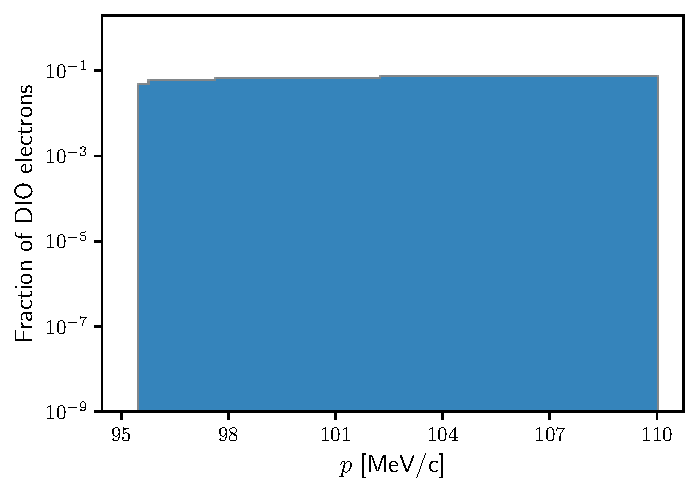
\includegraphics[width=\textwidth]{chapter6/dio_momentum_distribution_initial.pdf}
    \caption{Initial sampling.}
\end{subfigure}
    \hspace{2cm}
    \begin{subfigure}[t]{0.4\textwidth}
        \centering
        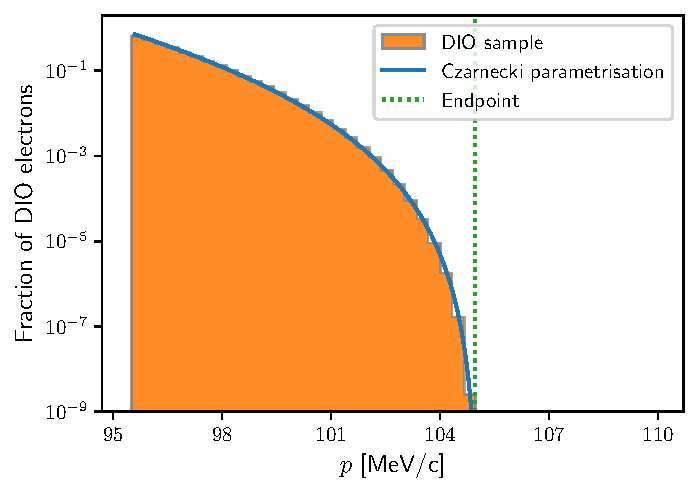
\includegraphics[width=\textwidth]{chapter6/dio_momentum_distribution_czarnecki_weighted.pdf}
        \caption{Weighted with the Czarnecki et al. parametrisation~\cite{czarnecki}.}
    \end{subfigure}
    \caption{Momentum spectrum of electrons in the DIO sample.}
    \label{fig:czarnecki_spectrum}
\end{figure}

The theoretical energy spectrum of DIO electrons produced in aluminium muonic
atoms was investigated by Czarnecki et al.~\cite{czarnecki}. Here, we use their
proposed parametrisation of the energy spectrum around the DIO energy endpoint:
\begin{equation}\label{eq:czarnecki_param}
P(E_e) = a_5 \delta^5 + a_6 \delta^6 + a_7 \delta^7 + a_8 \delta^8,
\end{equation}
where $\delta \equiv E_\mu  - E_e - \frac{E_e^2}{2 m_\mathrm{Al}}$, $E_\mu =
\SI{105.194}{\MeV}$, $m_\mathrm{Al} = \SI{25133}{\MeV}$, with the values of the
four $a$ coefficients they provide. This approximation is valid in the region
$E_e > \SI{85}{\MeV}$, which is sufficient to cover our whole DIO sample. We
use this spectrum parametrisation to weight DIO events based on their energy.
Similarly to the position weighting procedure, DIO events are first generated
with a uniform energy distribution in the range $p \in [95,
110]~\si{\MeV/\clight}$, and then weighted according to the probability for a
DIO electron to have the sampled energy. Figure~\ref{fig:czarnecki_spectrum}
shows the momentum spectrum of DIO electrons before and after weighting.

The DIO sample is composed of $N_\mathrm{DIO} = 10^7$ events in total.
Figure~\ref{fig:muon_dio_in_cydet} shows an example of a potential background
event from DIO where an electron with an energy close to the conversion energy
flies into the CyDet system and induces a trigger.

\begin{figure}
    \centering
    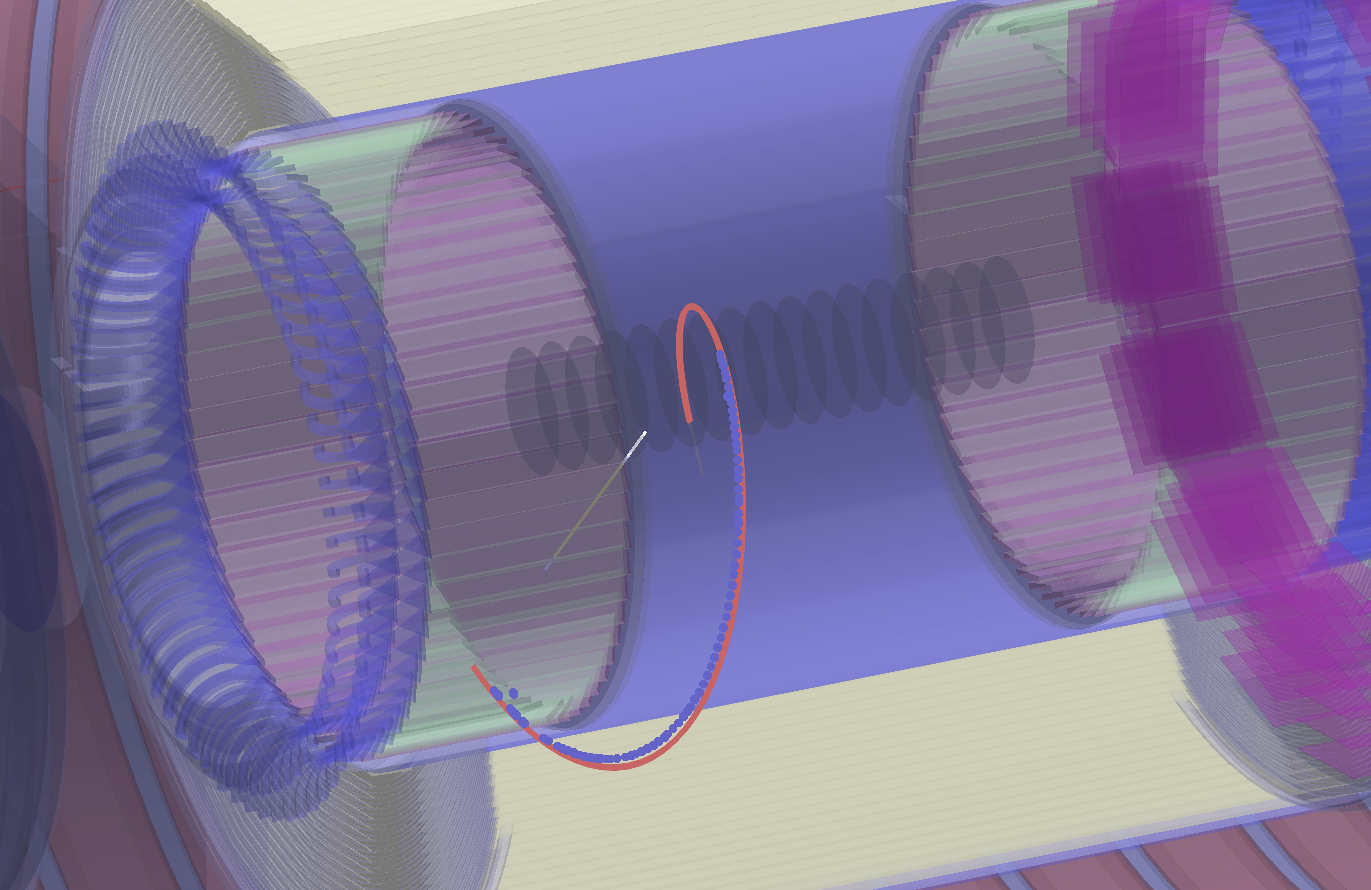
\includegraphics[width=0.6\textwidth]{chapter6/dio_event_in_cydet.png}
    \caption{Potential DIO-induced background with momentum $p=\SI{102}{\MeV/\clight}$.}
    \label{fig:muon_dio_in_cydet}
\end{figure}

\subsubsection{Selection}
The selection of DIO events is identical to the selection of conversion events.
We require a fourfold coincidence in the CTH, and then apply a Gaussian smear to
the true momentum of the electron to approximate track reconstruction. The same
efficiency and acceptance factors as for signal events are applied to weight the
sample and determine the absolute background contribution from the DIO process.


\subsection{Atmospheric muons}

\subsubsection{Sample}

Atmospheric muon events are simulated as discussed in
Section~\ref{sec:cosmic_event_sampling}. Two samples are produced, one around the
entire surface of the CRV and one more densely concentrated on its upstream and
downstream openings. Because of how rarely a sampled atmospheric event produces
signal-like features, the atmospheric dataset is the largest of the three, with
$1 \times 10^9$ events generated on the envelope and $1.4 \times 10^9$ on the
openings.



\begin{figure}
    \centering
    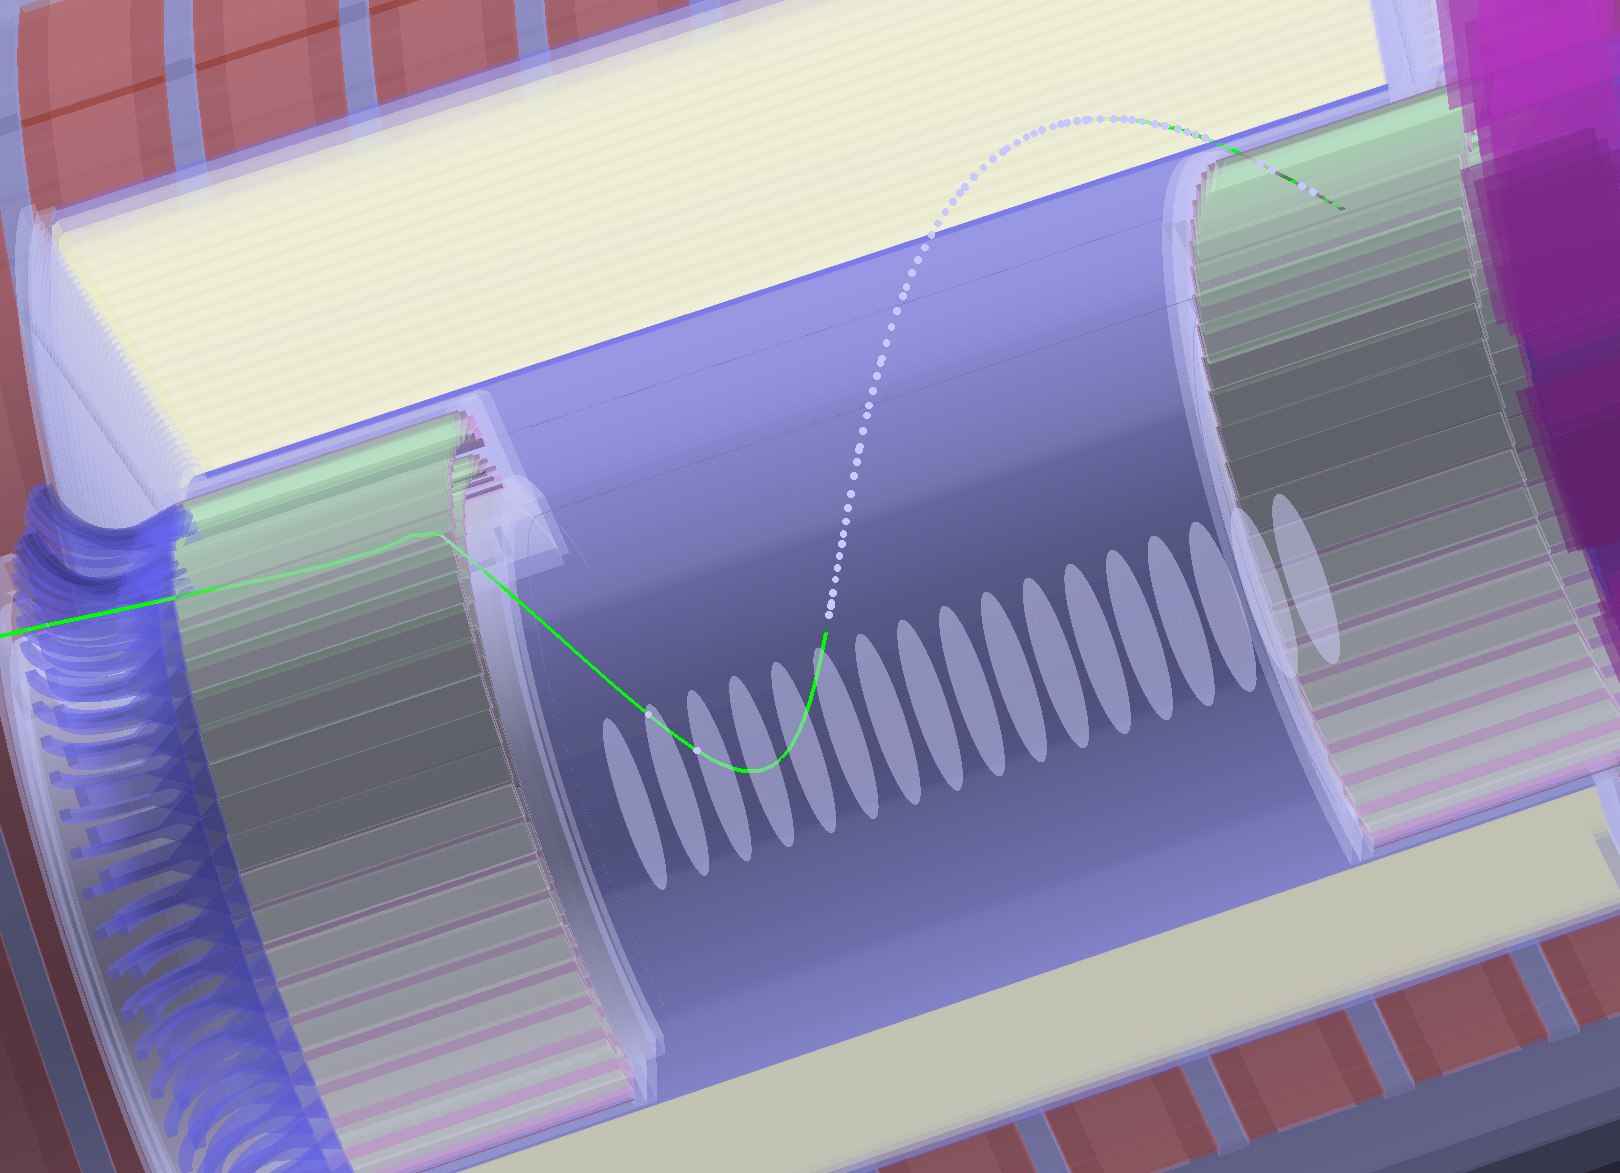
\includegraphics[width=0.6\textwidth]{chapter6/atmospheric_event_in_cydet.png}
    \caption{Cosmic ray-induced background with momentum
    $p=\SI{101}{\MeV/\clight}$. \hl{What particle type is it? What true/fitted
    momentum does it have? Where does it enter, first interact to create this
    signal-like track?}}
    \label{fig:cosmic_bg_in_cydet}
\end{figure}

\subsubsection{Selection}
As for signal and DIO events, atmospheric events must at least pass the fourfold
coincidence criterion. Unlike signal and DIO events, hit information from the
CDC is also used to select track candidates. Two criteria apply: the particle
must reach at least the 5th innermost layer of the CDC, but it should not hit
the outermost layer. Hence, we select tracks with sufficient transverse
momentum to be reconstructed, but reject tracks that either have too large a
momentum to be a signal event, or appear to enter the CDC from the outside. 

In addition, the hit positions are used to reconstruct the track using a helix
fit. The fitted trajectory should intersect the muon stopping target to pass the
selection. Figure~\ref{fig:cosmic_bg_in_cydet} shows an example of an
atmospheric event that would pass this selection. The helix fit estimates the
momentum of the particle, which is used in the analysis stage. Hence, for this
sample, we do not apply a Gaussian smear to the true momentum but use the
estimated momentum from the fit instead.

\subsubsection{Rate estimation}
As discussed in Section~\ref{sec:bmc_conversion_bg_rate}, the rate for each selected
event is estimated by backward MC simulation. The backward propagation and flux
sampling is repeated 5000 times for every event, which yields an average flux
and a statistical error shown in the results.


\subsection{Sample weighting}\label{sec:sample_weighting}
\sepfootnotecontent{fn:conv_br_norm}{The nuclear muon capture branching ratio appears in this
expression because the branching ratio of $\mu$--$e$ conversion is
conventionally normalised to $\mathcal{B}_\mathrm{capture}$.}

Because they originate from different processes, the three MC samples must be
individually weighted in order to determine the absolute contribution from each.
The conversion and DIO processes both originate from the muons bound in the
stopping target, hence we can express the total number of expected conversion
and DIO electrons in terms of the total number of stopped muons $N_\mu$.
The number of signal electrons, as a function of the conversion branching
ratio $\mathcal{B}_\mathrm{conversion}$, is:
\begin{equation}\label{eq:weight_signal}
N_\mathrm{conversion} = 
N_\mu \, \mathcal{B}_\mathrm{conversion} \, 
\mathcal{B}_\mathrm{capture} \, f_\mathrm{coherent},
\end{equation}
where $\mathcal{B}_\mathrm{capture} = 0.61$ is the branching ratio of nuclear
muon capture\sepfootnote{fn:conv_br_norm} and $f_\mathrm{coherent}=0.9$ is the
fraction of conversions that are coherent.

Similarly, the total number of DIO electrons can be expressed as:
$$
N_\mathrm{DIO} = N_\mu \, \mathcal{B}_\mathrm{DIO},
$$
where $\mathcal{B}_\mathrm{DIO} = 1 - \mathcal{B}_\mathrm{capture} = 0.39$ is
the branching ratio of DIO. Our simulation sample, however, only covers the part
of the DIO spectrum where $E_e > \SI{95}{\MeV}$, so we cannot simply use
$N_\mathrm{DIO}$ as the sample weight. The proper weight is given by 
\begin{align}\label{eq:weight_dio}
N_\mathrm{DIO}^{p>\SI{95}{\MeV}} &= N_\mathrm{DIO} \, P(E_e > \SI{95}{\MeV}) \\\nonumber
&= N_\mathrm{DIO}\,\int_{\SI{95}{\MeV}}^{E_\mathrm{endpoint}} P(E_e)\,dE_e,
\end{align}
where $E_\mathrm{endpoint} = \SI{104.973}{\MeV}$ is the energy above which no
DIO electron can be produced. The integral term in this equation is estimated by
numerically integrating the Czarnecki parametrisation of
Equation~\ref{eq:czarnecki_param}.
%  to obtain $N_\mathrm{DIO}^{p>\SI{95}{\MeV}} = 0.67$ assuming $N_\mu = 1.5e16$.

In the case of atmospheric muons, the backward MC procedure yields an absolute
rate $R$ for each event. This rate can simply be integrated over the total
data acquisition time of the experiment $T_\mathrm{DAQ}$ to obtain the expected
event count:
\begin{equation}\label{eq:weight_atmospheric}
N_\mathrm{atmospheric} = \int_0^{T_\mathrm{DAQ}} R dt = R \times T_\mathrm{DAQ}.
\end{equation}

\hl{v This is still a lie... We say otherwise two paragraphs below.}

In this study, we use the value of $T_\mathrm{DAQ} = 146$~days required for
Phase-I to reach its sensitivity goal according to the TDR. This run time
corresponds to $N_\mu = 1.5 \times 10^{16}$. In the subsequent analysis, we
substitute these two values into
Equations~\ref{eq:weight_signal},~\ref{eq:weight_dio}
and~\ref{eq:weight_atmospheric} to weight each sample.



\subsubsection{Trigger time window efficiencies}
In order to take into account the trigger timing window, we assume that
atmospheric muons irradiate the detector with a uniform time distribution.
Hence, the time window efficiency factor is the average fraction of time when
the trigger is active:
$$
\epsilon_\text{time window}^\mathrm{atmospheric} =
\frac{8}{9}\,\frac{1170 - 700}{1170} = \SI{36}{\percent}
$$
assuming the trigger window is between 700 and \SI{1170}{\ns}, and where the
factor $\frac{8}{9}$ arises from the bunch structure of the J-PARC main ring. In
contrast, the efficiency factor for conversion and DIO electrons
$\epsilon_\text{time window}^\text{conversion|DIO} = \SI{30}{\percent}$ is
smaller because the time distribution of bound muons is not uniform but peaks
around \SI{300}{\ns}, before the trigger becomes active (see
Figure~\ref{fig:timing_distributions}).



\section{Single event sensitivity}
As discussed in Section~\ref{sec:SES}, the single event sensitivity (SES) is
defined as the value of the $\mu$--$e$ conversion branching ratio required for
the experiment to observe one signal event. It can be expressed in terms of the
experimental acceptance $A_{\mu-e}$ and the total number of muons stopped in the
stopping target $N_\mu$:
\begin{equation*}
\mathrm{SES} = 
\frac{1}{N_\mu\,A_{\mu-e}\,\mathcal{B}_\mathrm{capture}\,f_\mathrm{coherent}},
\end{equation*}
where $\mathcal{B}_\mathrm{capture} = 0.61$ and $f_\mathrm{coherent} = 0.9$.

In this simulation study, we found the geometrical acceptance $A_\mathrm{geom}$
of the CyDet with the new CTH layout to be reduced from \SI{26}{\percent} to
\SI{21}{\percent}. Hence, the net signal acceptance $A_{\mu-e}$ decreases from
\SI{4.1}{\percent} to \SI{3.3}{\percent}. On the other hand, the yield of
stopped muons per proton collision was also estimated from the MC5 dataset to be
$R_{\mu / p} = 4.86 \times 10^{-4}$, which is slightly higher than the TDR value
by a factor $1.03$. Overall, although the total number of bound muons is
increased for the same run time, it is outweighed by the decrease in acceptance.
Keeping $T_\mathrm{DAQ}$ fixed at 146 days, we obtain $N_\mu = 1.53 \times
10^{16}$, hence our estimation of the COMET Phase-I sensitivity is
$$
\mathrm{SES} = 3.61 \times 10^{-15}.
$$


\section{Analysis}

After applying the efficiency factors and weighting each sample by the total
number of expected events as per Section~\ref{sec:sample_weighting}, we are able
to determine the absolute contribution from each source over a given data
acquisition period.

\subsection{Momentum spectrum} %??

\begin{figure}
    \centering
        
    \begin{subfigure}[t]{0.49\textwidth}
        \centering
        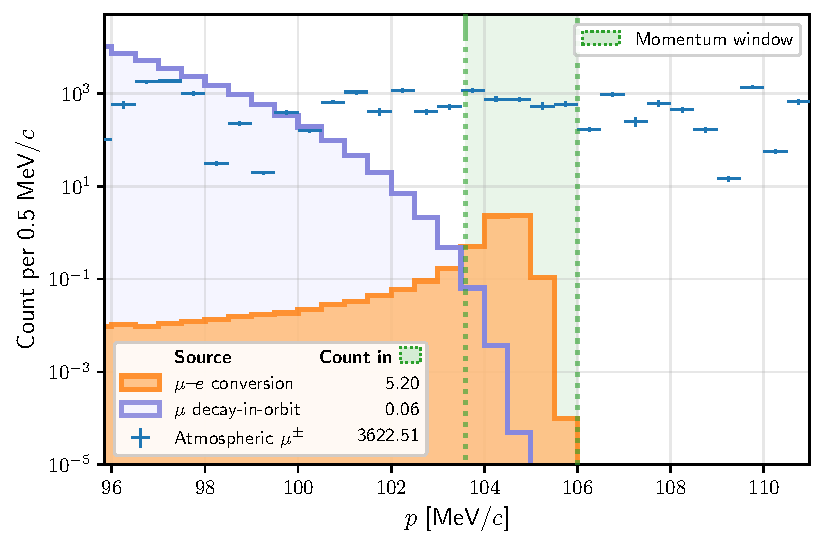
\includegraphics[width=\textwidth]{chapter6/thesis_conversion_search_momentum_distribution_nocuts_v5.pdf}
        \caption{ In the absence of event rejection by the CRV, the CTH trigger, and the timing window. }
        \label{fig:log_spectrum_nocuts}
    \end{subfigure}
    \hfill
    \begin{subfigure}[t]{0.49\textwidth}
        \centering
        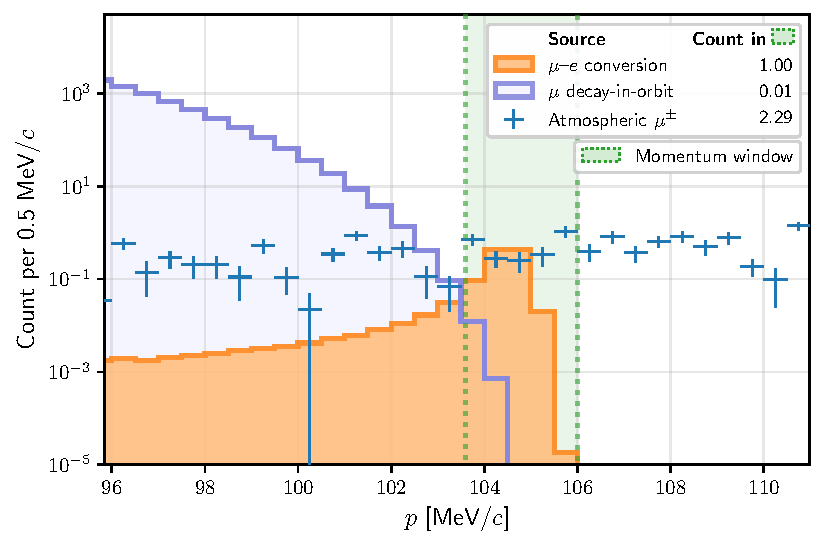
\includegraphics[width=\textwidth]{chapter6/thesis_conversion_search_momentum_distribution_withcuts_except_directionID.pdf}
        \caption{ With a \SI{99.99}{\percent}-efficient CRV. 
        }
        \label{fig:log_spectrum_cuts_except_directionID}
    \end{subfigure}
    \caption{ Momentum spectrum of conversion, DIO and atmospheric events around
    the conversion energy, integrated over the Phase-I run time $T_\mathrm{DAQ}
    = 146$~days, assuming $\mathcal{B}_\mathrm{conversion} = 3.61\times
    10^{-15}$. Error bars on the atmospheric event bins show the statistical
    uncertainty from the backward MC flux estimation.
    % For atmospheric events, we compare the absence and presence of
    % the CRV in rejecting backgrounds. We also show the effect of the time
    % trigger window and track quality cuts on the signal and DIO contributions. 
    }
    \label{fig:log_spectra}
\end{figure}


The absolute event counts from conversion, DIO and atmospheric muon events are
plotted as a function of the reconstructed track momentum in
Figure~\ref{fig:log_spectra}. Note again that for conversion and DIO, $p$ is the
smeared momentum of the electron as it enters the CDC, whereas we use the
momentum reconstructed via a helix fit for atmospheric muon events.


In order to determine the effect of the CRV on the atmospheric background, as in
Figure~\ref{fig:log_spectrum_cuts_except_directionID}, we apply a weight to each
event based on whether it passed through the active material of the CRV. For
events that produce hits in the CRV, the weight is the assumed inefficiency of
the CRV, $\epsilon_\mathrm{CRV} = 1 - \SI{99.99}{\percent} = 10^{-4}$. Events
that sneak into the detector are given a weight of 1 since the CRV cannot veto
them. Similarly, to simulate the absence of the CRV, as in
Figure~\ref{fig:log_spectrum_nocuts}, all atmospheric muon events have a weight
of 1, corresponding to a \SI{0}{\percent}-efficient CRV.



\sepfootnotecontent{fn:bg_study_rmc}{ We chose not to show the RMC spectrum in
    our plots because the contribution from RMC is smaller than that of DIO by a
    factor of 5~\cite{the_comet_collaboration_comet_2020}.}



% However, by investigating where
% these background events come from, we will see that there are ways to identify
% some of them and reduce their contribution below the single-event threshold.

The reconstructed momentum of the candidate track is one of the most important
criteria in discriminating signal electrons from DIO or
RMC\sepfootnote{fn:bg_study_rmc} electrons, because the energy spectra of the
latter two fall off sharply close to the conversion energy. In Phase-I, the
momentum window within which an event is counted is $p \in [103.6,
106.0]\,\si{\MeV/\clight}$. This cut eliminates the overwhelming majority of DIO
and RMC backgrounds. However, atmospheric background events appear to be uniformly
distributed in this region, making the cut ineffective in rejecting them. 

Figure~\ref{fig:log_spectrum_nocuts} shows that in the absence of the CRV,
atmospheric backgrounds overwhelm the detector and outnumber conversion events
by three orders of magnitude in the momentum window. In the presence of the CRV,
and assuming an efficiency of \SI{99.99}{\percent}
(Figure~\ref{fig:log_spectrum_cuts_except_directionID}), atmospheric backgrounds
are suppressed by a factor $10^3$. However, their integrated count still exceeds
one, making the $\mu$--$e$ conversion search impossible unless there is an
additional way to identify them.


% This is like a hard conclusion to swallow, should go at the end of the section
% so we can move straight to the ways in which we can try to identify atmos.


% For the atmospheric sample, we also reduce the background rate of certain events
% based on the primary particle ($\mu^-$ or $\mu^+$) and whether they hit the CRV.
% The first stage of the CTH, containing only scintillation counters and no
% Cherenkov counters, is unable to differentiate muons from electrons. Hence,
% signal-like tracks induced by sneaking atmospheric $\mu^+$ are a major source of
% backgrounds in this situation. 






\subsection{Particle identification}
%\subsection{Atmospheric \texorpdfstring{$\mu^+$}{anti-muon} backgrounds and particle identification}

In Figure~\ref{fig:log_spectrum_cuts_except_directionID}, we assumed that the
CyDet has no way of discriminating between electrons, muons, and anti-muons.
This is partly true since the first stage of the CTH will be composed of only
scintillation counters. These cannot help to identify the particle type like
Cherenkov counters, which are planned to replace one layer of scintillators in
the second stage of the CTH.

We investigate the effect of direction identification and CRV efficiency on the
background rate.

Positive muons can produce signal-like tracks in the CyDet by following the
reverse path of a conversion electron. Why? I have to explain exactly why.
Candidate signal electron trajectories originate in the muon stopping target,
produce a helical track in the CDC, and induce a fourfold coincidence in the
CTH. A $\mu^+$ can generate a background event by first hitting the CTH,
producing a track in the CDC, and then intersecting the muon stopping target,
appearing as a conversion track in reverse time ordering.

Question: if a mu+ follows the same time ordering as an e-, what does it look
like in the CyDet? 1. It curves in the other way as a negative particle in the B
field. Can that be easily rejected by the detector? At which step?

Paragraph: the stage-1 CTH can't do PID. Explain why, using Cherenkov counter
properties vs plastic scintillator.

Paragraph: reverse-direction mu+ track can still be identified via
time-of-flight information. Method was investigated internally by Moritsu, who
determined that direction identification method can reject 89 percent of
atmospheric mu+ events with, but reduces the net signal acceptance by a
factor 0.87.



\subsection{CRV efficiency}

\begin{figure}
    \centering
    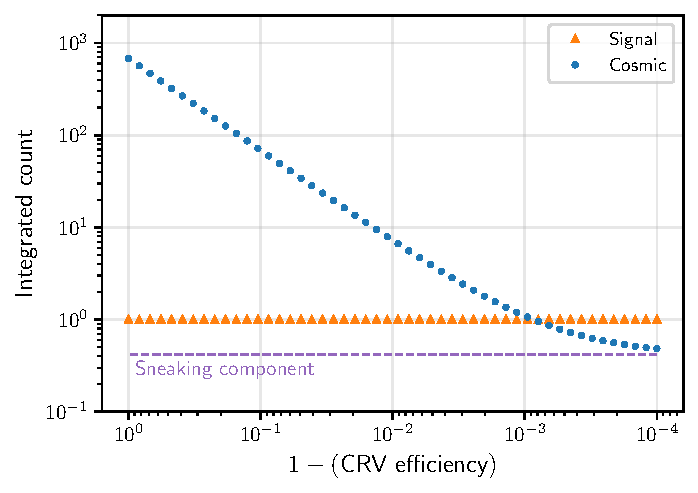
\includegraphics[width=0.5\textwidth]{chapter6/bg_count_vs_crv_efficiency.pdf}
    \caption{ Integrated atmospheric background count as a function of the CRV
        efficiency. The lower bound arises from sneaking events which cannot be
        identified by the CRV. More accurate particle identification by the
        CyDet helps to reduce this sneaking component, e.g.\ by discriminating
        muons from electrons.}
    \label{fig:bg_count_vs_crv_efficiency}
\end{figure}

The CRV efficiency determines the fraction of atmospheric events which
can enter the CyDet through the active parts of the CRV while not being vetoed.
Although we have assumed so far that the CRV is \SI{99.99}{\percent}
efficient, it will not necessarily be the case in practice.

Note that the portion of background events produced by atmospheric muons
sneaking through the CRV openings is unaffected by how efficient the CRV is.
These backgrounds can only be reduced by increasing the coverage of the CRV,
which has inherent limitations since the beam must enter on one side and exit
on the other.
